\documentclass[a4paper]{article}
\usepackage[utf8]{inputenc}
\usepackage{float}
\usepackage{pdfpages}
\usepackage{textcomp}
\usepackage{indentfirst}

\setlength{\parskip}{1em}

% Colour Management
\usepackage{color}

% Multi-Line Comments
\usepackage{comment}

% Customisable Sections
\usepackage{titlesec}

% Images and Captions
\usepackage{graphicx}
\usepackage{subcaption}
\usepackage{wrapfig}
\graphicspath{{./images/}}
\usepackage{fancyhdr} 


% Bibliography
\usepackage[nottoc]{tocbibind}
\usepackage[
    backend=biber,
    style=ieee]{biblatex}

\addbibresource{report_citations.bib} %Imports bibliography file


% Tables
\usepackage{xcolor}
\usepackage{array}
\newcolumntype{L}{>{\raggedright\arraybackslash}m{0.9\linewidth}}

% Contents Page
\usepackage{hyperref}

% Appendices
\usepackage[toc,page]{appendix}

% Bold Maths Symbols
\usepackage{bm}

% Allowing lower levels of Contents Page
\setcounter{tocdepth}{4}
\setcounter{secnumdepth}{5}

% Make margins smaller, feel free to change
\usepackage{geometry}
\geometry{
    a4paper,
    top = 20mm,
    bottom = 20mm,
    textwidth=426pt
}





\title{Engineering Design Project}
\author{Georgio Chaimali \and 
        Dimitrios Georgakopoulos \and 
        Edvard J. Skaarberg Holen \and 
        Hyunjoon Jeon \and 
        Josiah Mendes \and 
        Raghav Viswakumar}
\begin{document} 
\begin{titlepage}
    \setlength{\headheight}{66.89pt}
    \thispagestyle{fancy}
    \renewcommand{\headrulewidth}{0pt}
    \renewcommand{\footrulewidth}{0pt}
    \lhead{
\includegraphics[scale=0.1]{logo.png}}
    \cfoot{} % this is to remove the page number
    \hbox{}\vfill
    \begin{center} 
	    {\scshape\LARGE Imperial College London  \par}
	    \vspace{1cm}
        {\scshape\Large Second Year Design Project\par}
        \vspace{0.25cm}
        {\scshape\Large ELEC50003/ELEC50008\par}
        \vspace{1.5cm}
        {\huge\bfseries The MARS Rover\par}
        \vspace{2cm}
        {\Large\itshape Group 1\par}
        \vfill
        \begin{flushright}
            \textsl{ \large
            Georgio Chaimali \\ 
            Dimitrios Georgakopoulos \\ 
            Edvard J. Skaarberg Holen \\ 
            Hyunjoon Jeon \\ 
            Josiah Mendes \\ 
            Raghav Viswakumar
            }
        \end{flushright}
        \vfill

        % Bottom of the page
        {\large Word Count: XXXX Words \\ \today\par}
    \end{center}
\end{titlepage}
 

\tableofcontents

\newpage

\section{Overview}

\section{Systems}

\subsection{Control}
\subsection{Comms}

\subsection{Vision}
\begin{abstract}
    The purpose of the Vision module is threefold:
    1. Capture data from camera module;
    2. Detect objects of interest within the current view and 
        send their location to the Control module; and
    3. Send image data to Control for streaming to Command. 
\end{abstract}

\subsubsection{Hardware Organisation}

The Vision module comprises of two main hardware elements: 
    the Terasic DE10-Lite, a cost-effective Intel MAX 10 based FPGA board 
    \cite{TerasicDE10Web} 
    and the Terasic D8M-GPIO camera package \cite{TerasicD8MWeb}
that interfaces with the FPGA through the onboard GPIO connectors. 

These hardware choices were made by the project organisers, 
but are also sufficient and capable of carrying out the tasks at hand. 
As the FPGA's hardware is configurable, 
it is more flexible than other embedded systems 
that are limited to a general purpose processor,and 
is also able to handle both streaming and processing of high resolution images
without significant compromises on framerate or data speed 
through the use of concurrent operations and dedicated blocks 
for signal processing applications like multiplication.
This particular FPGA is also equipped with a 4-bit VGA output 
which is useful for debugging object detection live, 
and also has a connector for an Arduino Uno R3 shield, \cite{TerasicDE10Web} 
which can be used to interface with the ESP32 used for control.  

In order to perform general purpose operations like
    to configure camera settings
    and to provide a debugging interface,
a Nios II soft core was instantiated on the FPGA. 
Alternatively, to implement a more advanced image processing algorithm
or to reduce other hardware components in the system like the multiple Arduinos, 
a FPGA with a hard core, 
known as a FPGA System-On-Chip (FPGA SoC) \cite{FPGASoC} could be used, 
which would provide both the advantages of having reconfigurable hardware 
and a more capable general purpose processor. 

\subsubsection{Image Capture Processing Stream}

The image capture and buffering is based on a starter project provided
by Terasic Inc for the D8M Camera module that was modified by Ed Stott 
\cite{EEE2Rover}. 



\subsection{Drive}

% Start of energy subsection
\subsection{Energy}
\begin{abstract}
The main goal of the energy sub-module is to design a battery pack for the rover and charge it using solar power. With this goal in mind, the energy sub-module must develop a battery management system which allows the tracking of battery SOC and SOH, and if necessary perform SOH maintenance. 
    
\end{abstract}

\subsubsection{Characterising Components}
When designing a system it is necessary to know the behaviour and limitations of its constituent components. There are three main components that make up the energy subsystem: the battery cells, the PV panels and the SMPS.

\textbf{\chapter{Battery Cells}}
\newline
\newline
To determine the behaviour of the battery cells they were all tracked through a full charge/discharge 
cycle using the provided “Battery\_Charge\_Cycle\_Logged\_V1.1.ino” code\cite{clemow}. 
Every cell behaved similarly in terms of the cell voltage compared to time. 
The cell voltage of cell 1 over a full discharge/charge cycle is shown in figure~\ref{fig:charge_cycle}:

\begin{figure}[H]
    \centering
    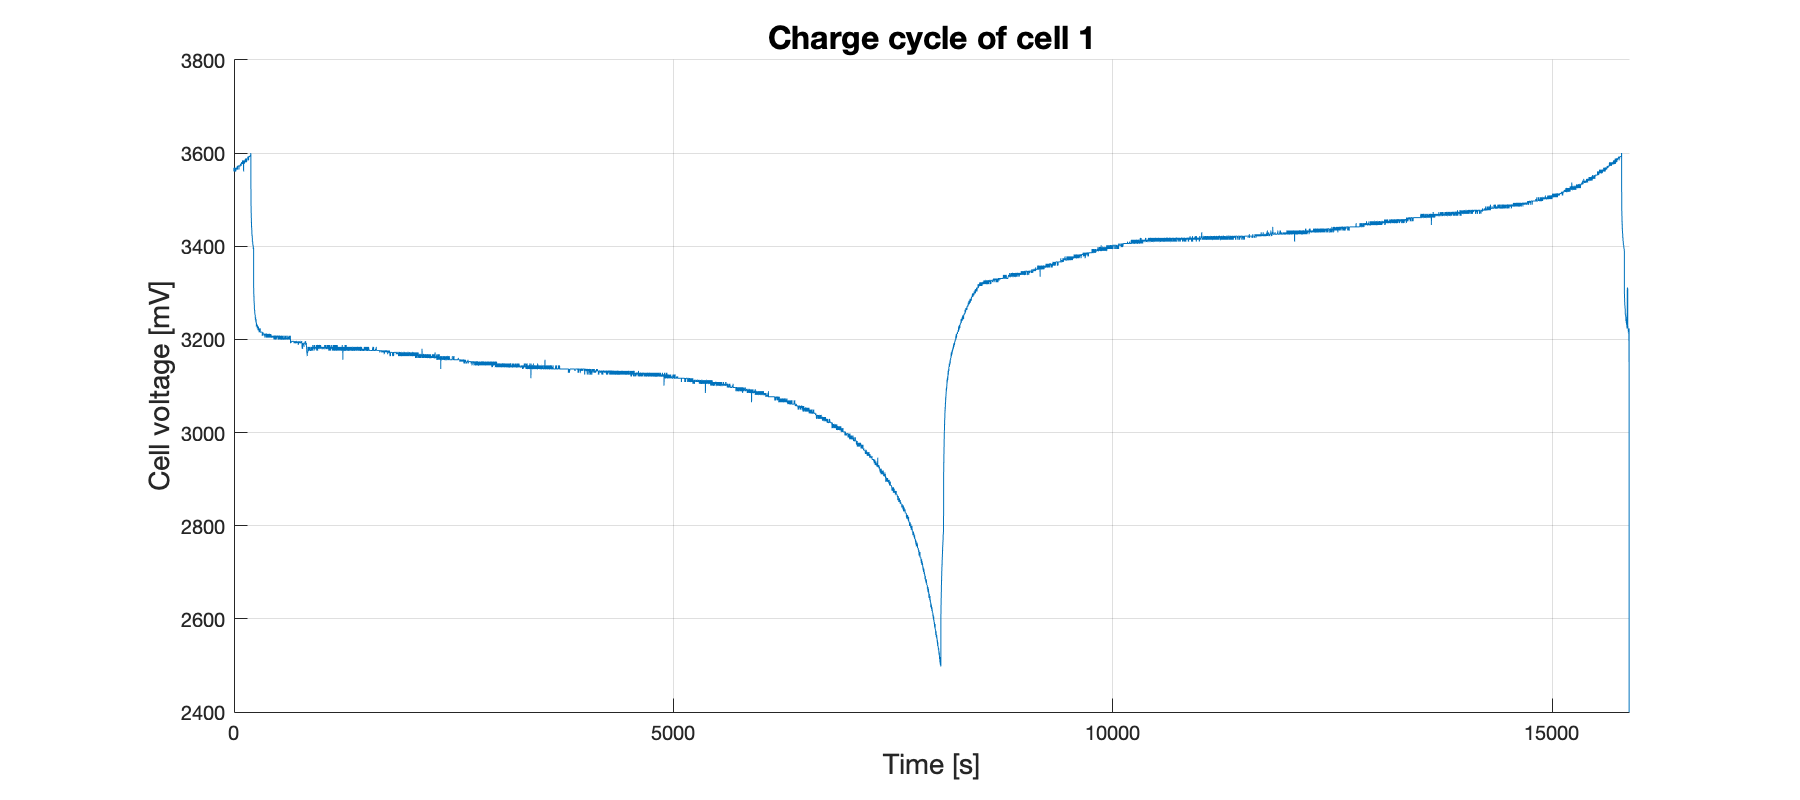
\includegraphics[scale=0.18]{charge_cycle.png}
    \caption{The voltage evolution of cell 1 through a full discharge/charge cycle.}
    \label{fig:charge_cycle}
    \end{figure}

Note the following important points on the graph. At 200 s the cell is done charging and
enters an idle state for 30 s after which it starts discharging. At ~8000 s the cell is fully
discharges and enters an idle state for 30s after which it starts charging. Finally, at 18800 s the cell is once 
again fully charged and the charge cycle is completed.

The provided charging algorithm also logs the current into the cell.
By integrating said current for a full charge or discharge section
we can determine the cell capacity in mAh. The results of this analysis is 
presented in the table below:

\begin{center}
    \begin{tabular}{||c| c c c c c||} 
    \hline
   Cell Number& 1 & 2 & 3 & 4 & 5 \\ [0.5ex] 
    \hline
    Capacity (mAh) & 542.7	& 526.1	& 519.5	& 530.1	& 543.7\\ [1ex] 
    \hline
   \end{tabular}
   \end{center}


As expected all cells have a capacity somewhere around 500 mAh. However, some cells
are have a higher capacity than others which may have implications for the performance
of certain battery cell configurations.

\textbf{\chapter{PV panels}} 
\newline
\newline
The provided PV panels are rated for a maximum power of 1.15 W at a voltage 
of 5.0 V and current 230 mA. Away from the maximum power point the performance of 
the panels can be determined from their I-V curves. To find the I-V curves each 
panel was connected to the B-inputs of the SMPS operating in non-synchronous boost.
They were then lit by the lamp and the duty cycle of the SMPS was varied while measurements 
of panel current and voltage were taken. After processing the resulting data
is plotted in figure~\ref{fig:IV_curve}.

 \begin{figure}[H]
    \centering
    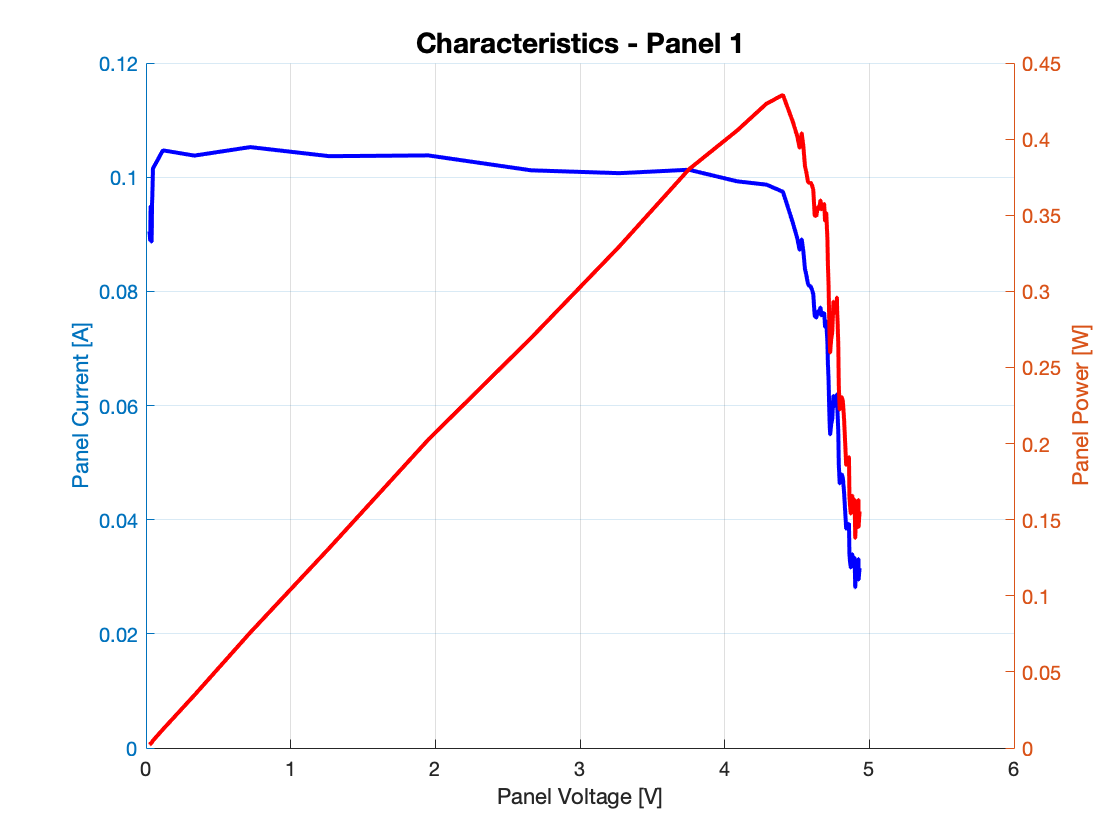
\includegraphics[scale=0.18]{Panel1.png}
    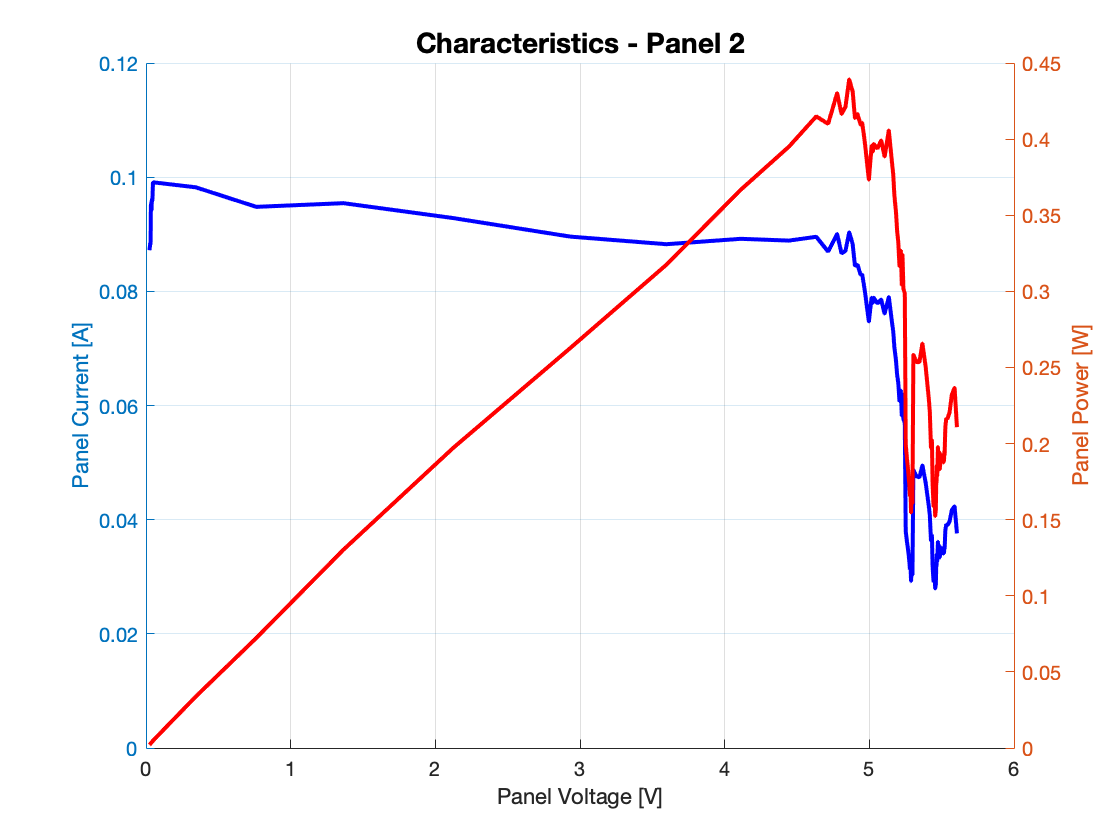
\includegraphics[scale=0.18]{Panel2.png}
    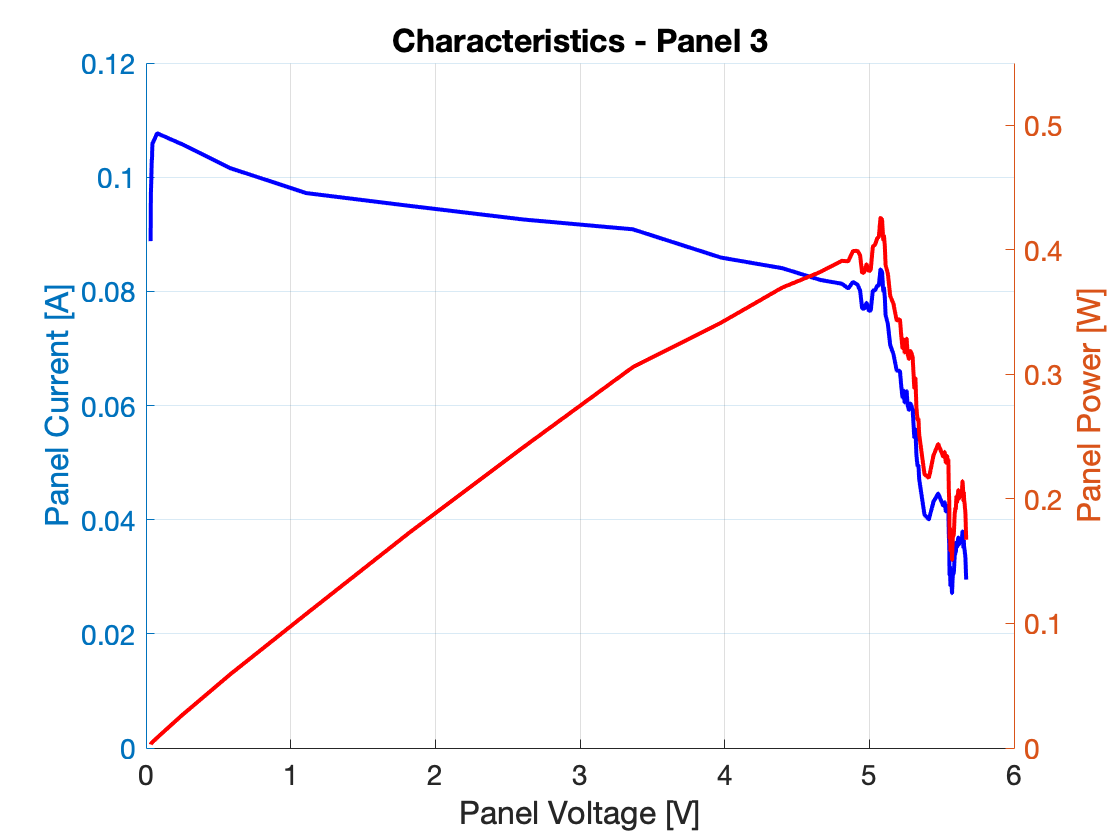
\includegraphics[scale=0.18]{Panel3.png}
    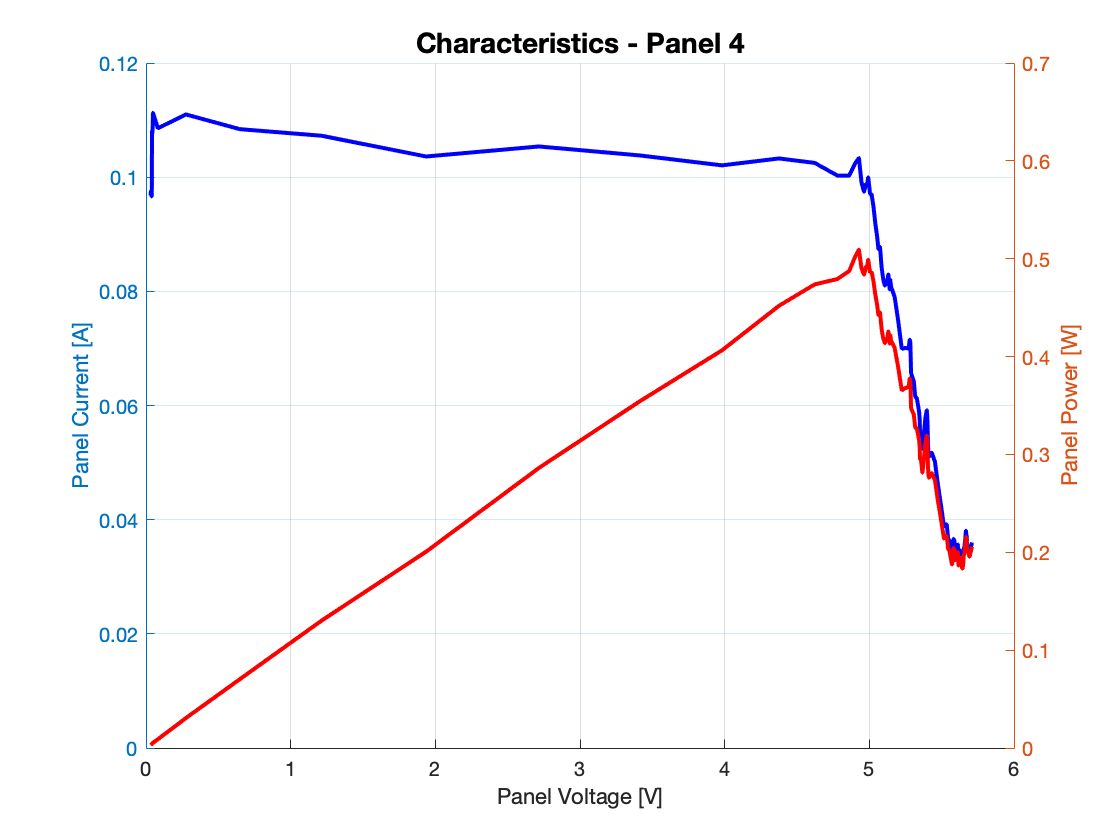
\includegraphics[scale=0.18]{Panel4.png}
    \caption{I-V curves for the PV panels.}
    \label{fig:IV_curve}
    \end{figure}

Though the data is noisy, it is clear that all panels exhibit the standard 
I-V characteristics of a PV cell. That is, they behave as non-ideal current 
sources with a nearly constant current at low voltages and a rapid current 
reduction at high voltages\cite{green}. Moreover, we see that the provided lamp activates 
the panels poorly as the peak power for each of the panels is only ~0.5 W.

\textbf{\chapter{SMPS}} 
\newline
\begin{wrapfigure}{r}{0.5\textwidth}
    \begin{center}
      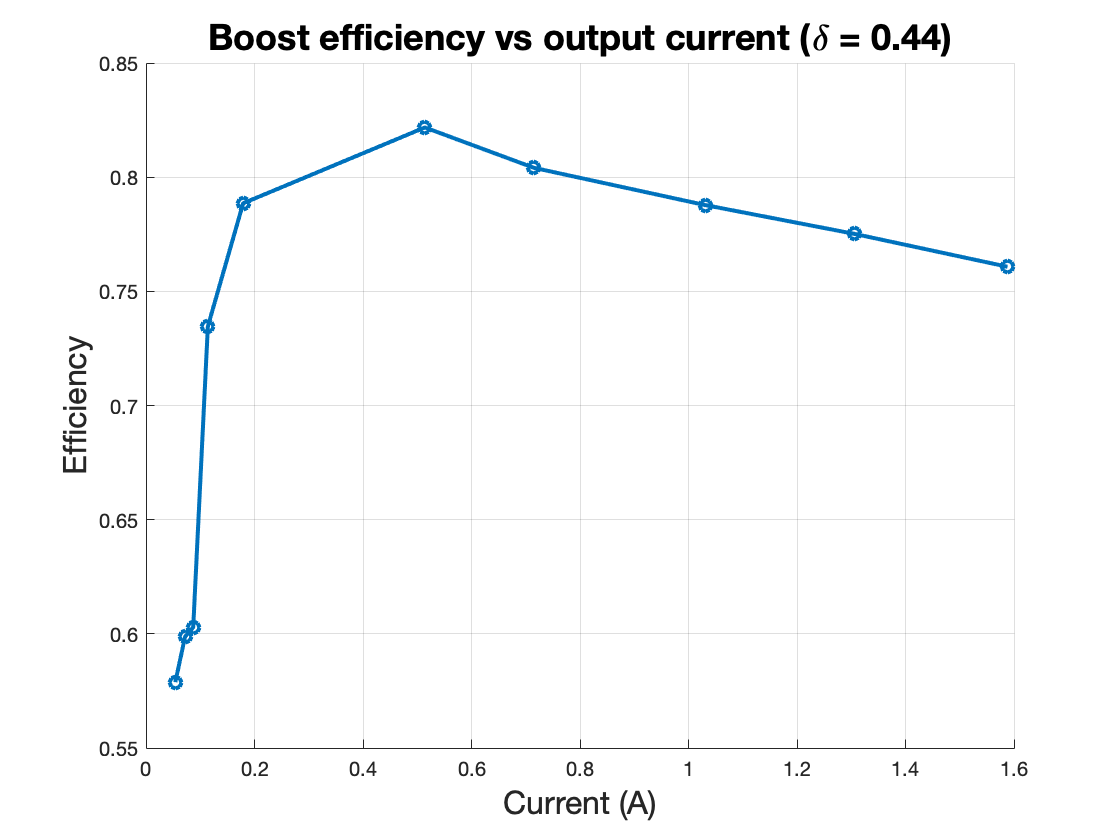
\includegraphics[width=0.48\textwidth]{Boost_efficiency_wduty.png}
    \end{center}
    \caption{SMPS efficiency versus output current with input voltage 5V}
    \label{fig:efficiency}
  \end{wrapfigure}
The provided SMPS is rated for 10 W throughput with a maximum boost output voltage of 35 V 
and maximum output current of 10 A\cite{SMPS_lab}. All these ratings are far higher 
than needed and neither is expected to impose limitations on the design of the energy module. 

The many characteristics of the SMPS have been thoroughly examined in 
2nd year labs. However, for the energy submodule the most important characteristics 
will be the SMPS efficiency during non-synchronous boost operation. A graph of 
efficiency versus output current is shown in figure~\ref{fig:efficiency}.


\subsubsection{Battery Configuration}

\subsubsection{PV Array Configuration}
    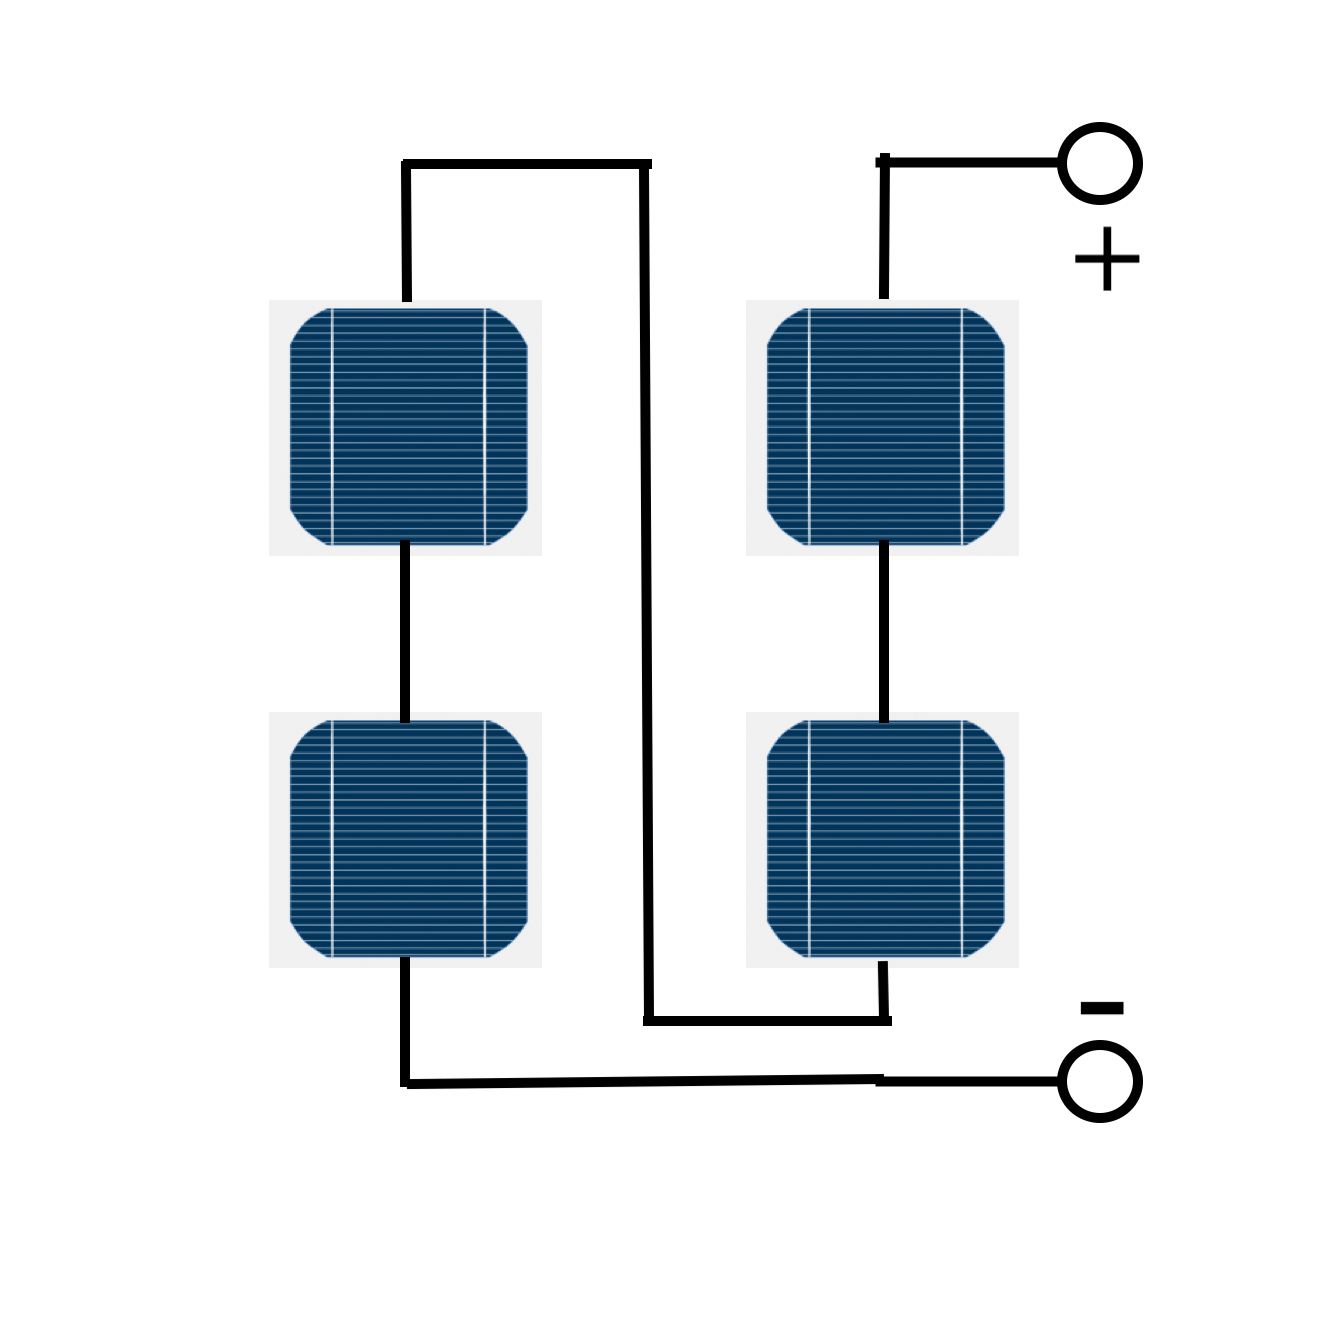
\includegraphics[scale=0.3]{Series(S)}

\subsubsection{SMPS Configuration}

\subsubsection{Maximum Power Point Tracking}

\subsubsection{Charging Algorithm}

\subsubsection{Discharging Algorithm}

\subsubsection{Safety Mechanisms}

\subsubsection{State of Charge}

\subsubsection{State of Health}
maintenance

\subsubsection{Communicating with Other Modules}
Though it is not necessary to fully integrate the energy module with the rest of the rover, other submodules, specifically command, needs access data such as the battery SOH and SOC. For communicating with other modules the Arduino shield has a set of UART ports. However, as group members were not in the same location it was not possible to physically connect the energy module to the rover, which is necessary to use UART. As such, an alternative approach was employed. First the Arduino was connected to a computer via USB. On the computer a Python script was run [8]. At the start the Python script establishes a connection to a server created by running a similar script on the command module [9]. After a connection has been established the Python script starts reading the serial data coming from the Arduino and transmits it using TCP to the command module. Each message coming from the Arduino is in CSV form where the first entry is the message ID, which allows the command script to decode what type of data is being sent. 

\subsubsection{Physical Integration of the Energy Module}

% End of energy subsection

\subsection{Integration}



\section{Evaluation and Conclusion}

\section{Project Management and Organisation}

As this project was carried out remotely
with contributors located in different countries, 
it was important to have a good framework for communication and management. 

The main tool used for communications and management was Git + GitHub.
As the codebase was incredibly complex, 
involving many different libraries and with each submodule being capable as a
standalone project, it was vital to have a version control system in place. 
Being able to keep a history of commits and changes made to a project was useful,
especially when trying to track down the origin of a bug and what caused it. 

The team also made use of GitHub Issues to track progress and accountability in 
the initial design phase. A thread was opened for each submodule to show what 
the lead for that submodule had been doing and potential avenues of achieving 
their goals. This was beneficial both for the leads to keep track of their 
research, but also allowed other members to contribute to other submodules 
by adding comments and voicing their thoughts. GitHub Issues were also linked 
directly to commits in the codebase to allow for a more in-depth explanation and
reasoning with context for a commit than what is allowed in the commit message 
area. 

Simultaneously, a Gantt chart was maintained to keep track of progress and is 
available for viewing under the maintained GitHub repository linked in the Appendix.

%TODO #7!
\section{Intellectual Property}

\newpage

\printbibliography[
heading=bibintoc,
title={References}
]


\begin{figure}[H]
\centering

\includegraphics[scale=0.18]{logo.png}
\caption{Sample Figure}
\label{fig:image1}
\end{figure}

Sample Reference\cite{einstein}


\begin{appendices}
\chapter{Some Appendix}
The contents...
\end{appendices}

\end{document}